\documentclass[11pt,a4paper]{article}
\usepackage[a4paper, portrait, margin=1in]{geometry}
\usepackage[utf8]{inputenc}
\usepackage[T1]{fontenc} 
\usepackage{graphicx}
\usepackage{booktabs}
\usepackage{enumitem}
\usepackage{pdfpages}
\usepackage{mathptmx}
\usepackage{anyfontsize}
\usepackage{titlesec}
\usepackage{tabto}
\usepackage{listings}

%\usepackage[table,xcdraw]{xcolor}
% If you use beamer only pass "xcolor=table" option, i.e. \documentclass[xcolor=table]{beamer}
\usepackage[normalem]{ulem}
\useunder{\uline}{\ul}{}

\usepackage{xcolor}

\definecolor{codegreen}{rgb}{0,0.6,0}
\definecolor{codegray}{rgb}{0.5,0.5,0.5}
\definecolor{codepurple}{rgb}{0.58,0,0.82}
\definecolor{backcolour}{rgb}{0.95,0.95,0.92}

\lstdefinestyle{mystyle}{
    backgroundcolor=\color{backcolour},   
    commentstyle=\color{codegreen},
    keywordstyle=\color{magenta},
    numberstyle=\tiny\color{codegray},
    stringstyle=\color{codepurple},
    basicstyle=\ttfamily\footnotesize,
    breakatwhitespace=false,         
    breaklines=true,                 
    captionpos=b,                    
    keepspaces=true,                 
    numbers=left,                    
    numbersep=5pt,                  
    showspaces=false,                
    showstringspaces=false,
    showtabs=false,                  
    tabsize=2
}

\lstdefinelanguage{JavaScript}{
  keywords={typeof, new, true, false, catch, function, return, null, catch, switch, var, if, in, while, do, else, case, break},
  keywordstyle=\color{blue}\bfseries,
  ndkeywords={class, export, boolean, throw, implements, import, this},
  ndkeywordstyle=\color{darkgray}\bfseries,
  identifierstyle=\color{black},
  sensitive=false,
  comment=[l]{//},
  morecomment=[s]{/*}{*/},
  commentstyle=\color{purple}\ttfamily,
  stringstyle=\color{red}\ttfamily,
  morestring=[b]',
  morestring=[b]"
}

\lstdefinelanguage{XML}
{
  morestring=[b]",
  morestring=[s]{>}{<},
  morecomment=[s]{<?}{?>},
  stringstyle=\color{black},
  identifierstyle=\color{blue},
  keywordstyle=\color{cyan},
  morekeywords={xmlns,version,type}
}
\lstset{language=C++,
                keywordstyle=\color{blue},
                stringstyle=\color{red},
                commentstyle=\color{green},
                morecomment=[l][\color{magenta}]{\#}}

\lstset{style=mystyle}

\usepackage{tocbasic}

\DeclareTOCStyleEntry[
  entrynumberformat=\entrynumberwithprefix{\figurename},
  dynnumwidth,
  numsep=1em
]{tocline}{figure}
\newcommand\entrynumberwithprefix[2]{#1\enspace#2:\hfill}

\usepackage{hyperref}
\hypersetup{
  colorlinks,
  allcolors=.,
  urlcolor=blue,
}

\usepackage{setspace}
\setcounter{secnumdepth}{4}
\titleformat{\paragraph}
{\normalfont\normalsize\bfseries}{\theparagraph}{1em}{}
\titlespacing*{\paragraph}
{0pt}{3.25ex plus 1ex minus .2ex}{1.5ex plus .2ex}

\usepackage{tikz}
\usepackage{amsmath}
\usetikzlibrary{shapes.geometric, arrows}
\usepackage{verbatim}
\usepackage{array}
\usepackage{caption}
\pagestyle{plain}
\setlength{\parindent}{0pt}
\renewcommand{\thesection}{\arabic{section}}

\hyphenpenalty 1000
\exhyphenpenalty 1000


\begin{document}

\begin{titlepage}

    \begin{center}
    
        {\fontsize{22}{27}\selectfont Department of Electronic and Telecommunication Engineering} 
	\vspace{\baselineskip}
	\vspace{\baselineskip}
        {\fontsize{20}{24}\selectfont \\Internet of Things}  
        {\fontsize{16}{19}\selectfont \\EN3250} 
    \vspace{\baselineskip}
	\vspace{\baselineskip}
        {\fontsize{20}{24}\selectfont \\Currency Converter Service}  
	   {\fontsize{18}{21}\selectfont \\Project Report\\} 
%		\vspace{\baselineskip}
%		\vspace{\baselineskip}   
%		\vspace{\baselineskip}
%		\vspace{\baselineskip}
		\vspace{\baselineskip}
    \end{center}

   \begin{center}
        
\includegraphics[width=0.4\textwidth]{images/uom.png}
    \end{center}
   \begin{center}   
      {\fontsize{16}{19}\selectfont University of Moratuwa\\}   
      \vspace{\baselineskip}
    \end{center}

\begin{flushleft}

{\fontsize{16}{19}\selectfont
\NumTabs{7}

\setlength{\itemindent}{1.7in}
\item 170258L 
      \tab
      :  R.H.R.  Jayarathne
\item 170543G
      \tab
      :  M.K.T. Sampath
 
\item 170698J
      \tab
      :  L.T.A. Wijayaratne

\item 170375R
      \tab
      :  D.R. Marasinghe


}
\end{flushleft}


\begin{center}
\vspace{\baselineskip}
\vspace{\baselineskip}
\vspace{\baselineskip}
\vspace{\baselineskip}
\vspace{\baselineskip}
\vspace{\baselineskip}
\vspace{\baselineskip}


 {\fontsize{10}{13}\selectfont This report is submitted in partial fulfilment of the requirements for the module}\\
  {\fontsize{10}{13}\selectfont EN3250 - Internet of Things}
 \end{center} 

\end{titlepage}



 




	

\pagenumbering{roman} 
\spacing{1.45} 
\newpage
\tableofcontents



\newpage

\pagenumbering{arabic} 
%Remove below sections after completing
\spacing{1.2}

\section{Introduction}

\subsection{Overview}

Foreign exchange market is a global market, where people around the world buy and sell different foreign currencies everyday for various purposes. One purpose of the traders in the market is engaging in day-trading activities, and is performed by normal people who intend to gain profits and earn from small price mismatches that are available for short time periods. Day traders’ activity is influenced by historical fluctuations of foreign currency prices as well as the information gained from several technical indicators. These indicators are generated by performing various mathematical transformations on the time series charts of currency prices. This information is of much value for Day Traders and they usually buy this market information from their trusted services.\\

This project focuses on providing foreign exchange market day-traders, a set of useful information, by using a currency API that provides live currency prices of various currencies around the world. Usually, historical currency price data are provided freely on a daily basis only, but these rates change by minute values, every few seconds. Day traders require these fast changing values and must pay a considerable price to access this information. Therefore, by storing the live currency data in a Firebase Realtime database, we are able to provide more information to Day Traders and other users.\\

The users of our application are able to log in using their email and password, and specify the currency type which they are interested in. Next, they are able to specify maximum (ceiling) and minimum (floor) values for the exchange rate (as a percentage of the exchange rate at the time of request) and receive notifications when the currency price crosses either of these thresholds. The notifications will be sent via emails as well as by a  Buzzer, which would ring to notify the users. Therefore,  the notifications would reach the user at times when he/she is offline as well, through the Buzzer ringing. These ceiling and flow values allow Day Traders to evaluate the performance of their investment over time, without having to monitor the variation of exchange rates manually.\\

An LCD screen displays the exchange rates of 6 types of currencies as stated below.

\begin{enumerate}[itemsep=-1.7mm]

\item GBP - Great Britain Pound
\item JPY - Japanese Yen
\item USD - US Dollar
\item KWD - Kuwait Dinar
\item AUD - Australian Dollar
\item EUR - Euro

\end{enumerate}

The display is refreshed every 30 seconds and shows whether each exchange rate has increased or decreased over the last 30 seconds.\\

Since the foreign exchange market is an international market, it operates 24 hours a day and five days a week. However, during the weekend the market closes its trading activities. The functioning of this application is turned off an hour after the trading activities are closed for a particular week and reopened an hour before the trading activities are resumed for the following week.


\subsection{Objectives}

This project aims at making exchange rates of a user’s preference, freely available with updates at 30 second intervals. The overall platform with user authentication and live dashboards helps boost the activities currency markets.

\begin{itemize}[itemsep=-1.7mm]

\item Inform the user when the investment has exceeded a certain percentage of profit (ceiling) or diminished below a certain percentage of loss (floor), even when he/she is offline via an alarm. \item This will allow them to make quick decisions and responses regarding their investments.
To send detailed emails of the exchange rate behaviour at times when the thresholds have been crossed.
\item Display historical variations of currency exchange rates and several technical analysis charts through live dashboards. These help the Day-Traders make useful predictions.
\item To display rapid variations of currency exchange rates via an LCD display and whether the exchange rate has increased or decreased within the preceding 30 second interval.
\item Ensure that the NodeMCU, and the resource constrained devices in this application operate in an energy efficient manner.


\end{itemize}


\subsection{Scope}

The scope of the project includes an application using IOT concepts, tools and standards to provide timely information to Day Traders. This provides the users with the following.

\begin{enumerate}[itemsep=-1.7mm]
\item Exchange rate of 6 currencies - updated every 30 seconds
\item Buzzer and Email notifications when set thresholds for exchange rates are exceeded
\item A dashboard displaying the variations of exchange rate and Technical indicators over time (updated hourly).
\end{enumerate}

The basic components of which the application comprises are given below.

\begin{enumerate}[itemsep=-1.7mm]
\item \textbf{A realtime database} (using Google Firebase)
\item \textbf{An open-source API} providing currency exchange rates 
\item \textbf{A Node-Red Dashboard} to display variations of the four technical indicators
\item \textbf{A Buzzer} to notify the user when the set thresholds for exchange rates have been exceeded
\item \textbf{An LED Display}  to display exchange rate variations
\item \textbf{A Node-MCU}  for accepting requests of the human users as well as to send control signals to a Buzzer and the LED Display
\item \textbf{A client mobile phone} as the user interface
\end{enumerate}

The MQTT protocol is used to facilitate communication between NodeMCU and the Node-RED application. The deep sleep mode of the NodeMCU is used to save power of the NodeMCU and the other constrained devices, during the weekend hours when the forex market is closed.



\section{Methodology}

\subsection{Architecture}

\begin{figure}[h]
    \centering
      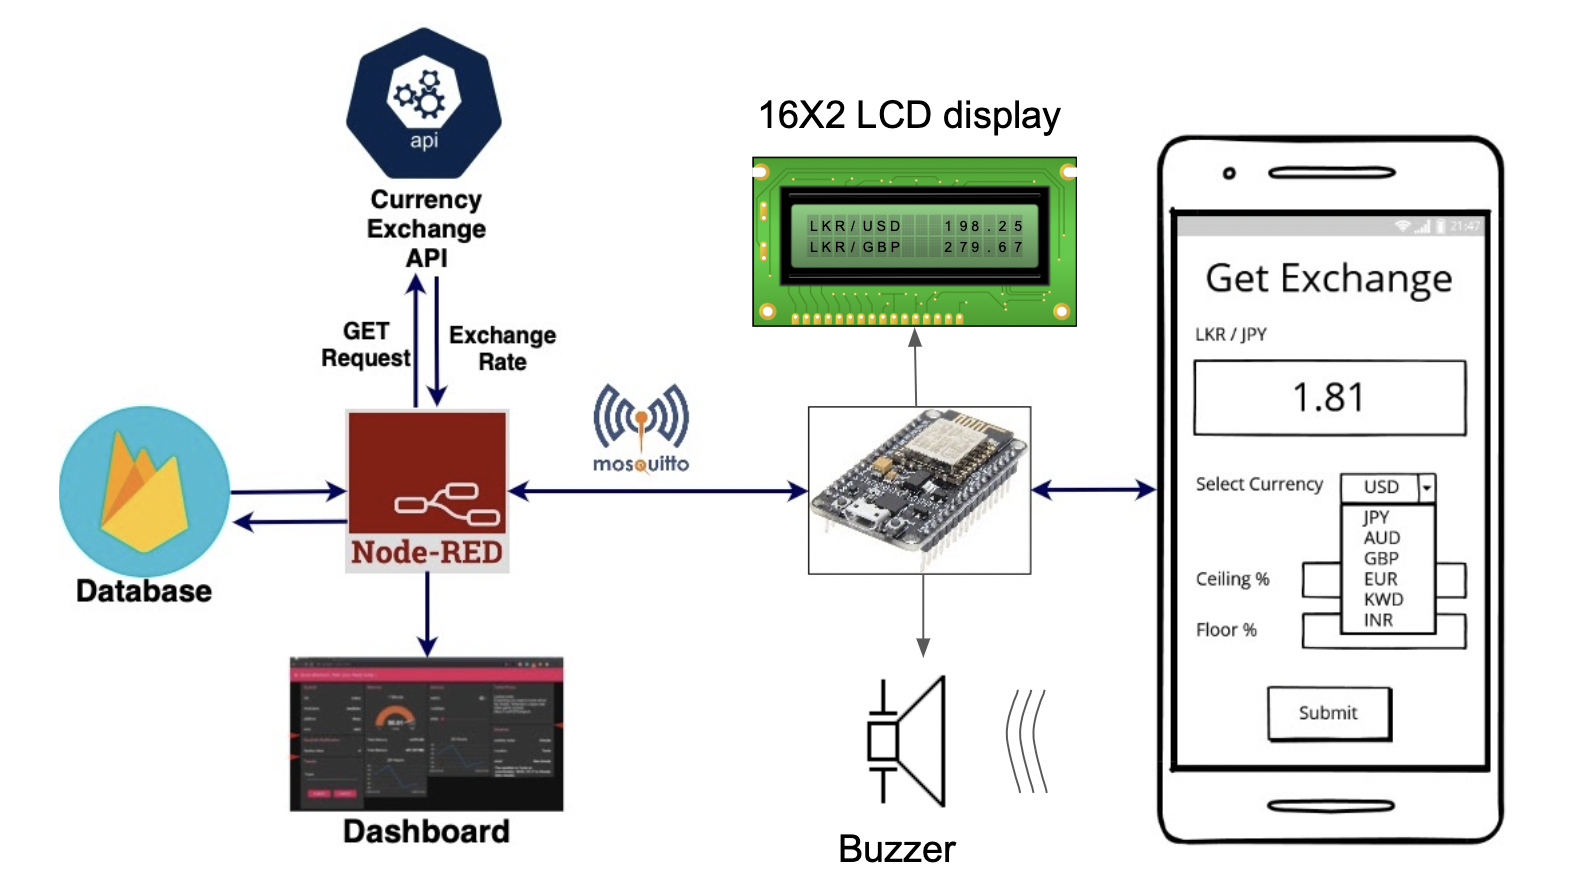
\includegraphics[width=1\textwidth]{images/arch.png}
    \caption{Architecture of the entire solution}
    \label{fig:arch}
\end{figure}

The login credentials of the users of this application are entered to the database from the backend by the database administrator. The user is able to log  in to the application using his/her mobile phone via a website hosted on a NodeMCU. The log in credentials are communicated to a Node-RED application via an MQTT broker and validated with the credentials stored in the Firebase database. On successful authentication, the Node-RED would publish a Success message token to admit the user.\\

Next, the user has the ability to select a currency of preference and specify the ceiling and floor thresholds. These values will also be communicated to the Node-RED application through a MQTT topic, and stored in the Firebase database.\\

A timer which is sending API requests at hourly intervals extracts the currency exchange rates and stores it in the database. The proposed architecture for this project requires exchange rate data every 30 seconds to accurately capture the minor changes in exchange rates, but the free version of the API only provides hourly exchange rate prices. We store these hourly exchange rates in the firebase database and use a gaussian random number generator to vary the hourly exchange rates by minor values to simulate rapid fluctuations of exchange rates similar to their real variations. The ceiling and floor values are checked against these simulated exchange rates at 30 second intervals, and if they are exceeded, an email is sent to the user. The exceeded message is sent to the NodeMCU via the MQTT broker and the Buzzer is sounded as well. This notifies the user in case he/she is offline.\\

The hourly exchange rate data is then used by the Node-RED application to calculate the following four technical indicators.\\

\begin{enumerate}[itemsep=-1.7mm]
\item Simple Moving Average (SMA)
\item Rate of Change oscillator (ROC)
\item Moving average convergence/divergence (MACD)
\item Relative Strength Index (RSI)
\end{enumerate}

These indicators calculated using exchange rate data over 40 hours are plotted on a live dashboard. 

\subsection{Functionalities of NodeMCU}

\begin{figure}[h]
    \centering
      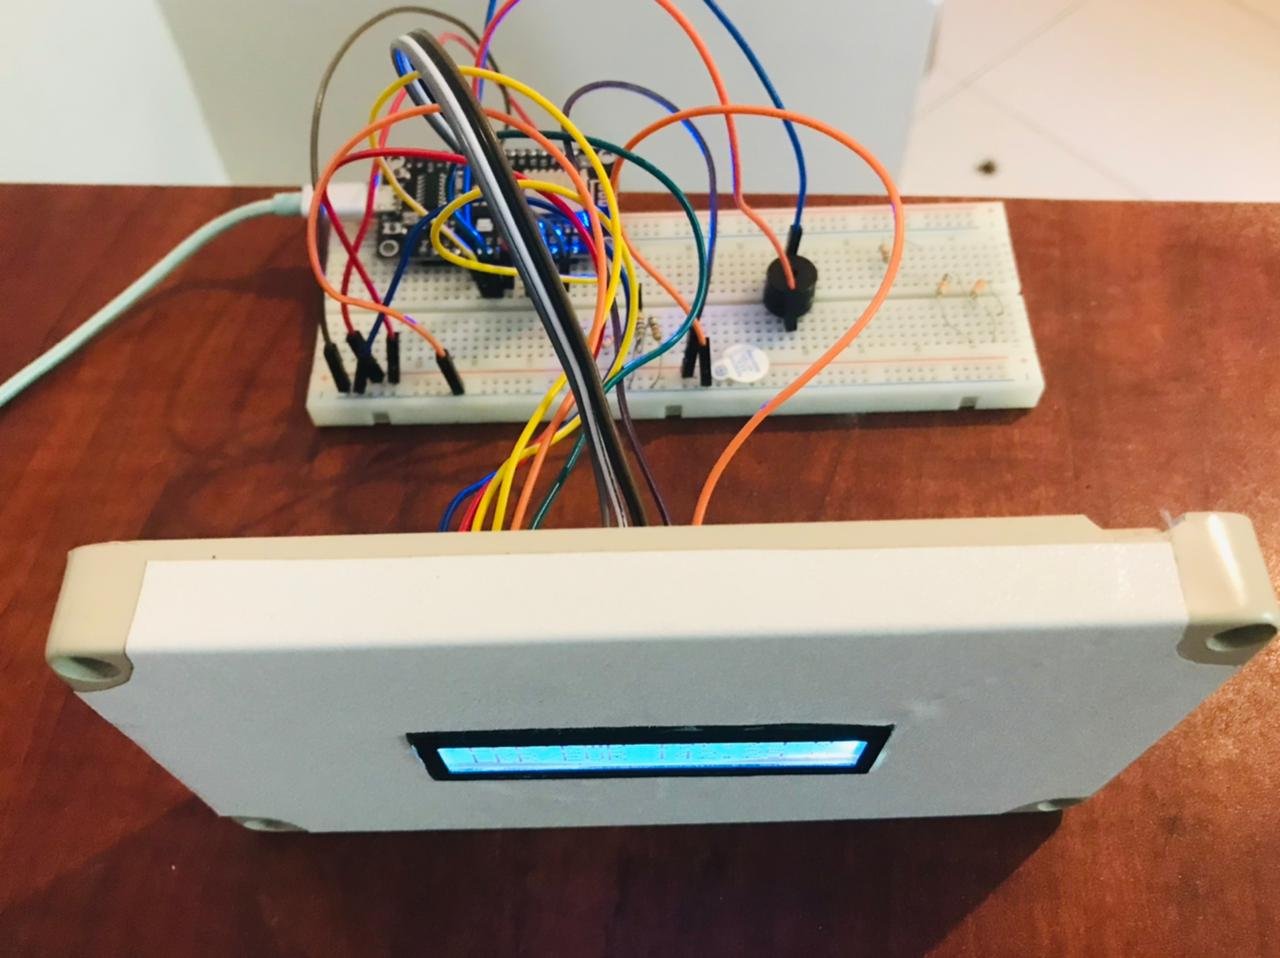
\includegraphics[width=0.7\textwidth]{images/front.png}
    \caption{Setting up ESP8266 with an LCD display and a buzzer}
    \label{front}
\end{figure}

The NodeMCU used in the IOT system performs multiple tasks to facilitate the connectivity between the user’s device, the LCD display, and the buzzer. ESP8266 NodeMCU was used in the testing process. The flow chart in the figure, describes the functionality of the NodeMCU.


\subsubsection{Hosting Web Interface for User}

\begin{figure}[H]
    \centering
      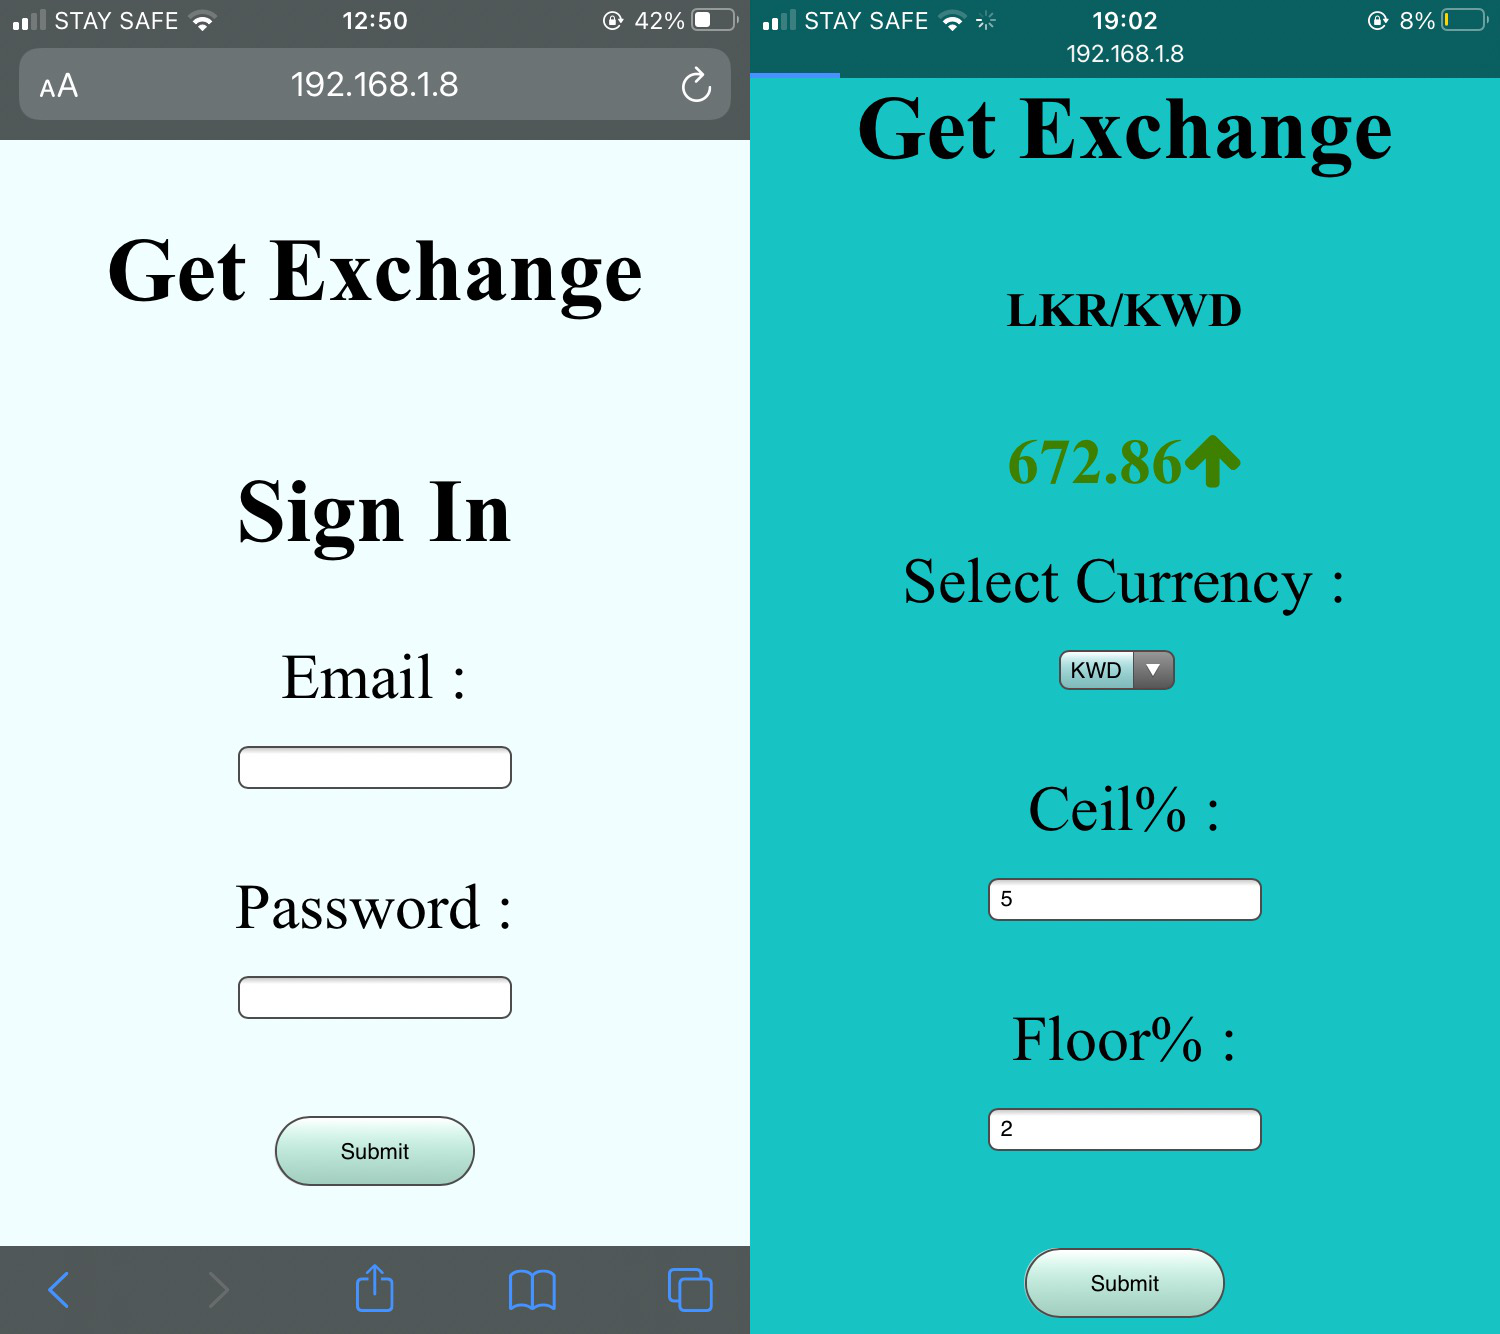
\includegraphics[width=0.4\textwidth]{images/login.png}
    \caption{Login page and home page for the user}
    \label{host}
\end{figure}

The above code calls two functions that return HTML scripts, which enable two HTML pages in figure  to be displayed. When the user loads 192.168.1.8 in the web browser, the login page on the left will appear in the mobile. After the authentication details are submitted, the user is redirected to the home page given that the authentication is successful.\\

In the home page. The user can select a preferred currency out of six available currencies. Additionally, the user can select two percentages to set the ceiling and floor prices compared to the current price. The current price of the selected exchange rate is then displayed on the home page.

\subsubsection{Authentication and authorization flow}

An authentication and an authorization flow is included in the IOT system. This flow is included in figure  . The first step of authentication is the initial login page that requests the user to enter an email and a password. After obtaining the username and the password, NodeMCU sends authentication data to Node-RED through MQTT. Node-RED acts as an authorization server and generates an application access token. This access token is sent back to the NodeMCU through MQTT. NodeMCU then stores the access token along with the user name. Whenever NodeMCU is sending user specific data to Node-RED, the access token is also sent along with it to verify the validity of the user.

\subsubsection{Setting up the MQTT Broker}

The Mosquitto MQTT \cite{mosq} server/broker was used to establish communications between the NodeMCU and the Node-RED application.The messages were published and received in the string data type and each component of the message was separated by a “\$” sign for encoding. This allows several types of information to be transmitted using a single message.\\

The NodeMCU subscribes to four MQTT topics (a., b., c., and d. below), and publishes to two MQTT topics (d., and e.).\\

\textbf{a. IOT\_6B/G05/UserAuth}\\

The login credentials of the user are sent to the Node-RED application for validation through this topic. The format of the published message is as follows.\\

timestamp\$user\_email\$password\\

\textbf{b. IOT\_6B/G05/AuthResponse}\\

The Nod-RED publishes the response status of the user authentication to this topic and is received by the NodeMCU. The format of the published message is as follows.\\

timestamp\$email\$status\$token\\
1623921792\$first.last@gmail.com\$success\$dhbasdg\\
1623921792\$first.last@gmail.com\$error\$null\\

\textbf{c. IOT\_6B/G05/UserNeeds}\\

The Nod MCU publishes the currency type subscribed to by a particular user, along with the ceiling and floor values requested for notifications. The format of the published message is as follows.\\

timestamp\$token\$currency\$ceil\_percentage\$floor\_percentage\\

\textbf{d. IOT\_6B/G05/UserNeedsResponse}\\

The response token from the Node-RED, stating the validity of the request message sent to the IOT\_6B/G05/UserNeeds topic, is published to this topic.  The format of the published message is as follows.\\

timestamp\$access\_token\$status\\
Status - success or error\\

\textbf{e. IOT\_6B/G05/CommonData} \\

This topic  receives the exchange rates of all 6 currency types and is updated every 30 seconds from the Node-RED. These values are received by the NodeMCU, and displayed on the LCD screen. The exchange rate of the selected currency type is displayed on the web interface for the user. The format of the published message is as follows.\\

timestamp\$USD\$GBP\$JPY\$AUD\$KWD\$EUR\$100101 \\
1623921792\$195.25\$145.25\$195.25\$145.25\$195.25\$145.25\$001101\\

\textbf{f. IOT\_6B/G05/BuzzerNotification} \\

Messages are published to this topic by the Node-RED application when the ceiling and floor prices, specified by the user, have been exceeded by the exchange rate. The format of the published message is as follows.\\

timestamp\$access\_token\$currency\$ceil\_bit\$floor\_bit\\
1623921792\$dhbasdg\$USD\$1\$0\\


The components of the encoded MQTT messages are as follows.

\begin{itemize}[itemsep=-1.7mm]

\item timestamp - Time at which the data is sent in Unix epoch format. This helps to validate timely data and to discard older messages.
\item ceil\_bit - A flag bit which is set to 1 if the ceiling price is crossed, else zero
\item floor\_bit - A flag bit which is set to 1 if the floor price is crossed, else zero
\item Bit stream - Each of the 6 bits corresponds to the 6 currency types and is set to 1 if there is an increase in the exchange rate, 0 otherwise.
\item access\_token - Indicates that the application is authorized to access user’s data \cite{token}

\end{itemize}


MQTT transmissions occur at random times, and the inclusion of the timestamp in the messages facilitated them to be checked to identify old messages. Those which took more than 20 seconds for transmission are discarded. Combining the data using this encoding scheme was required, because several components of the data are used at a certain instance. Further, this method of encoding and transmitting data allowed the LCD display to be updated in one transmission.\\

This simple encoding scheme allows more data to be transmitted with little overhead which can help reduce the power usage of the NodeMCU.

\newpage

\begin{figure}[H]
    \centering
      \includegraphics[width=1\textwidth]{images/overallmin.png}
    \caption{Complete technical process flow chart of the Methodology}
    \label{front}
\end{figure}

\newpage

\subsubsection{Decoding compact received data}

The goal here is to decode this large string containing several information components, separated using “\$” signs and to assign each of them to separate variables in the NodeMCU, as shown below. \\


1623921792\$200.25\$155.25\$1.82\$143.25\$197.25\$142.25\$101000\\


timestamp = 1623921792, USD = 200.25 , GBP = 155.25, JPY = 1.82, AUD = 143.25, KWD = 197.25 , EUR = 142.25\\

When a subscribed topic receives a data item, the \textbf{callback} function is called. The function considers the topic from which data is received and directs the data to the relevant purpose. For example, the \textbf{process\_notification}  function takes data from the \textbf{“IOT\_6B/G05/BuzzerNotification”} topic, \textbf{process\_Data} function takes data from the \textbf{“IOT\_6B/G05/CommonData”}, etc. An extract of the \textbf{callback} function is given below.\\

\begin{lstlisting}[language=C++]
void callback(char* topic, byte* payload, unsigned int length) {
  if (String(topic) == "IOT_6B/G05/BuzzerNotification") {
   process_notification(payload, length, 50, 5);
  }
  if (String(topic) == "IOT_6B/G05/CommonData") {
   process_data(payload, length, 70, 8);
  }
	:
	:
}
\end{lstlisting}

\vspace{\baselineskip}
The \textbf{process\_notification} function given below, splits the byte array into character arrays and then saves them in the variables treating them as separate cases, at every \textbf{callback} call.\\

\begin{lstlisting}[language=C++]
void process_notification(byte* payload, unsigned int length, int charlen, int numitem) {

     int digit;
     payloadstr = "";
     Serial.println();
     for (int i = 0; i < length; i++) {
       payloadstr += (char)payload[i];
     }

     char payloadstr_array[charlen];
     payloadstr.toCharArray(payloadstr_array, charlen);

     char * token = strtok(payloadstr_array, "$");
   
     for (int i = 1; i < numitem+1; i++) {
        switch (i) {
         case 1:
            timestamp = atol(token);
            Serial.print(timestamp);
            Serial.println();
            break;
	:
	:
         }
         token = strtok(NULL, "$");
     }
}
\end{lstlisting}

\subsubsection{Sensing alerts and notifying the user}

When an alert is sent through the \textbf{“IOT\_6B/G05/BuzzerNotification”} topic, the callback function instantly identifies a crossing in ceiling or floor prices, if any, and activates the \textbf{buzzer}. 
To identify notifications which have expired is essential, to ensure that the user is alerted based on timely information only. The NodeMCU was configured to be updated with the time and date so that it could be compared with the timestamp of received notification messages in unix epoch time format. A sample code is given below.\\

\begin{lstlisting}[language=C++]
if (timestamp > unix_epoch - 19820) {
    current_user = String(token);
}
\end{lstlisting}

\subsubsection{Supporting the LCD 16x2 display}

\begin{figure}[H]
    \centering
      \includegraphics[width=0.4\textwidth]{images/lcd.png}
    \caption{LCD display showing currency values time and date}
    \label{abcd}
\end{figure}


LCD display is used to show the live currency prices updated every 30 seconds, along with the date and time. These values are displayed one after the other, each being displayed for 2 seconds. The time and date was obtained using an available library (the NTPClient library) for NodeMCU, which enables it to communicate with an NTP (Network Time Protocol) Server.\\

\subsubsection{Power Saving Mechanisms of the NodeMCU}

The NodeMCU, along with the LCD display and the buzzer are power constrained devices. Hence power saving methods must be implemented to improve energy efficiency.\\

The main power saving method is by implementing the sleep function in the NodeMCU. When the Foreign exchange markets are closed during the weekends, the Node MCU enters the deep sleep mode to conserve power. Meanwhile, the dashboards from Node-RED are available for the user to monitor the exchange rate fluctuations. However, the maximum NodeMCU deep sleep time is 3 hours and 46 minutes \cite{deepsleep} and if the NodeMCU is kept in deep sleep mode for too long, it may stay in the sleep mode forever. The deep sleep mode is scheduled to begin 15 minutes after the time at which the Forex market is closed and then enters a series of sleep-wake-sleep cycles until 15 minutes before the market is set to open.\\

15 minutes after the market closes, the NodeMCU is set to sleep for an hour. Then it wakes up, and checks whether the market is open or closed using the current time and date. If it is closed, the NodeMCU goes back to sleep for another hour. This is continued till the market opens. NodeMCU is set to keep sleeping every week from Saturday 1.45 a.m. to Monday 2.15 a.m \cite{hours}.\\

The second power saving mechanism used in this application is the use of a simplified message encoding scheme in the form of a string of messages separated by “\$” signs. The same can be done using messages in JSON format, but this would require an additional library to be installed in the ESP8266, as well as a much larger overhead for the messages which are transmitted. The reduction of the message size in the encoding scheme suggested in this project actively reduces the power consumed in data transmission.


\subsection{Functionalities of the Node-RED Application}

Node-RED is a flow-based development tool which was used in this project to implement the backend functionalities, database connectivity, and live dashboards for this project.

\subsubsection{Extracting Data from the Exchange Rate API}

The Exchangeratesapi.io API service has been used to obtain the exchange rates of the selected 6 currency types. The API service used for this application is updated every second with the exchange rates of many types of currencies. For our application we proposed that exchange rates are needed to be sampled at 30 second intervals but a paid account is required with a fee up to USD 80.00 per month to obtain exchange rates at such a high frequency, as shown in the figure \ref{fig:exapi}.

\begin{figure}[H]
    \centering
      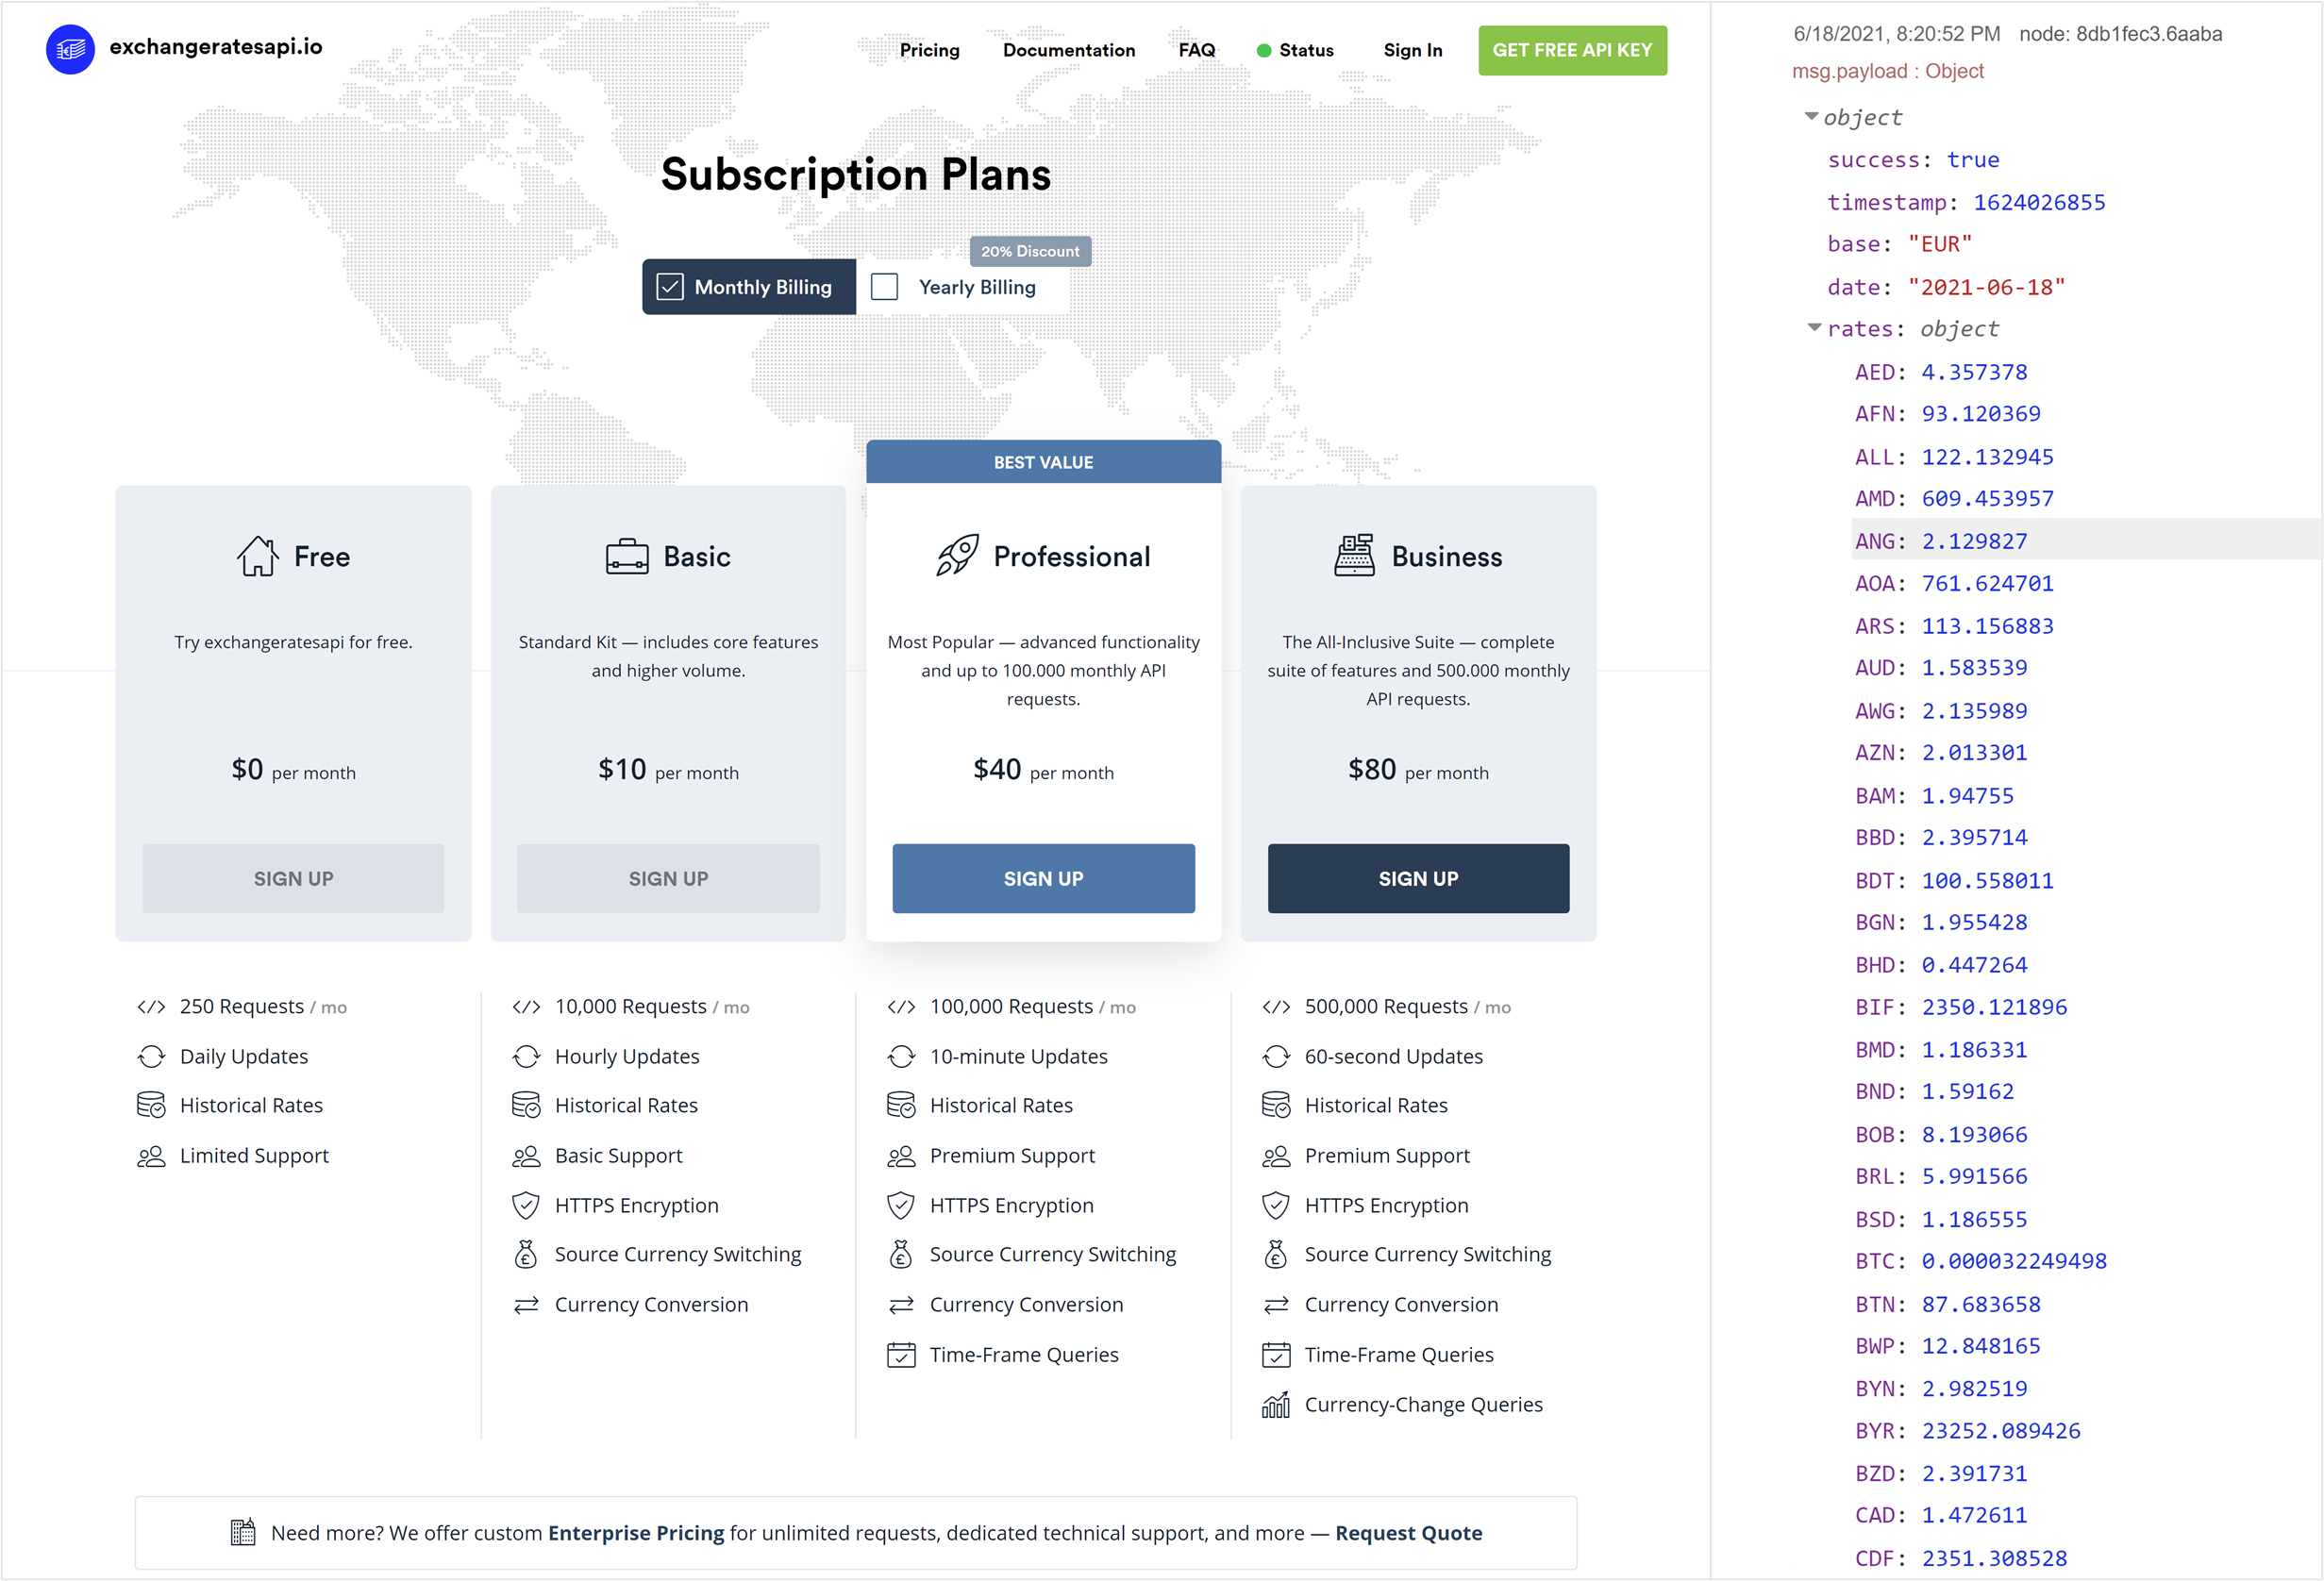
\includegraphics[width=1\textwidth]{images/exapi.png}
    \caption{The subscription plans of the API and the Response array containing Exchange rates}
    \label{fig:exapi}
\end{figure}

\begin{figure}[H]
    \centering
      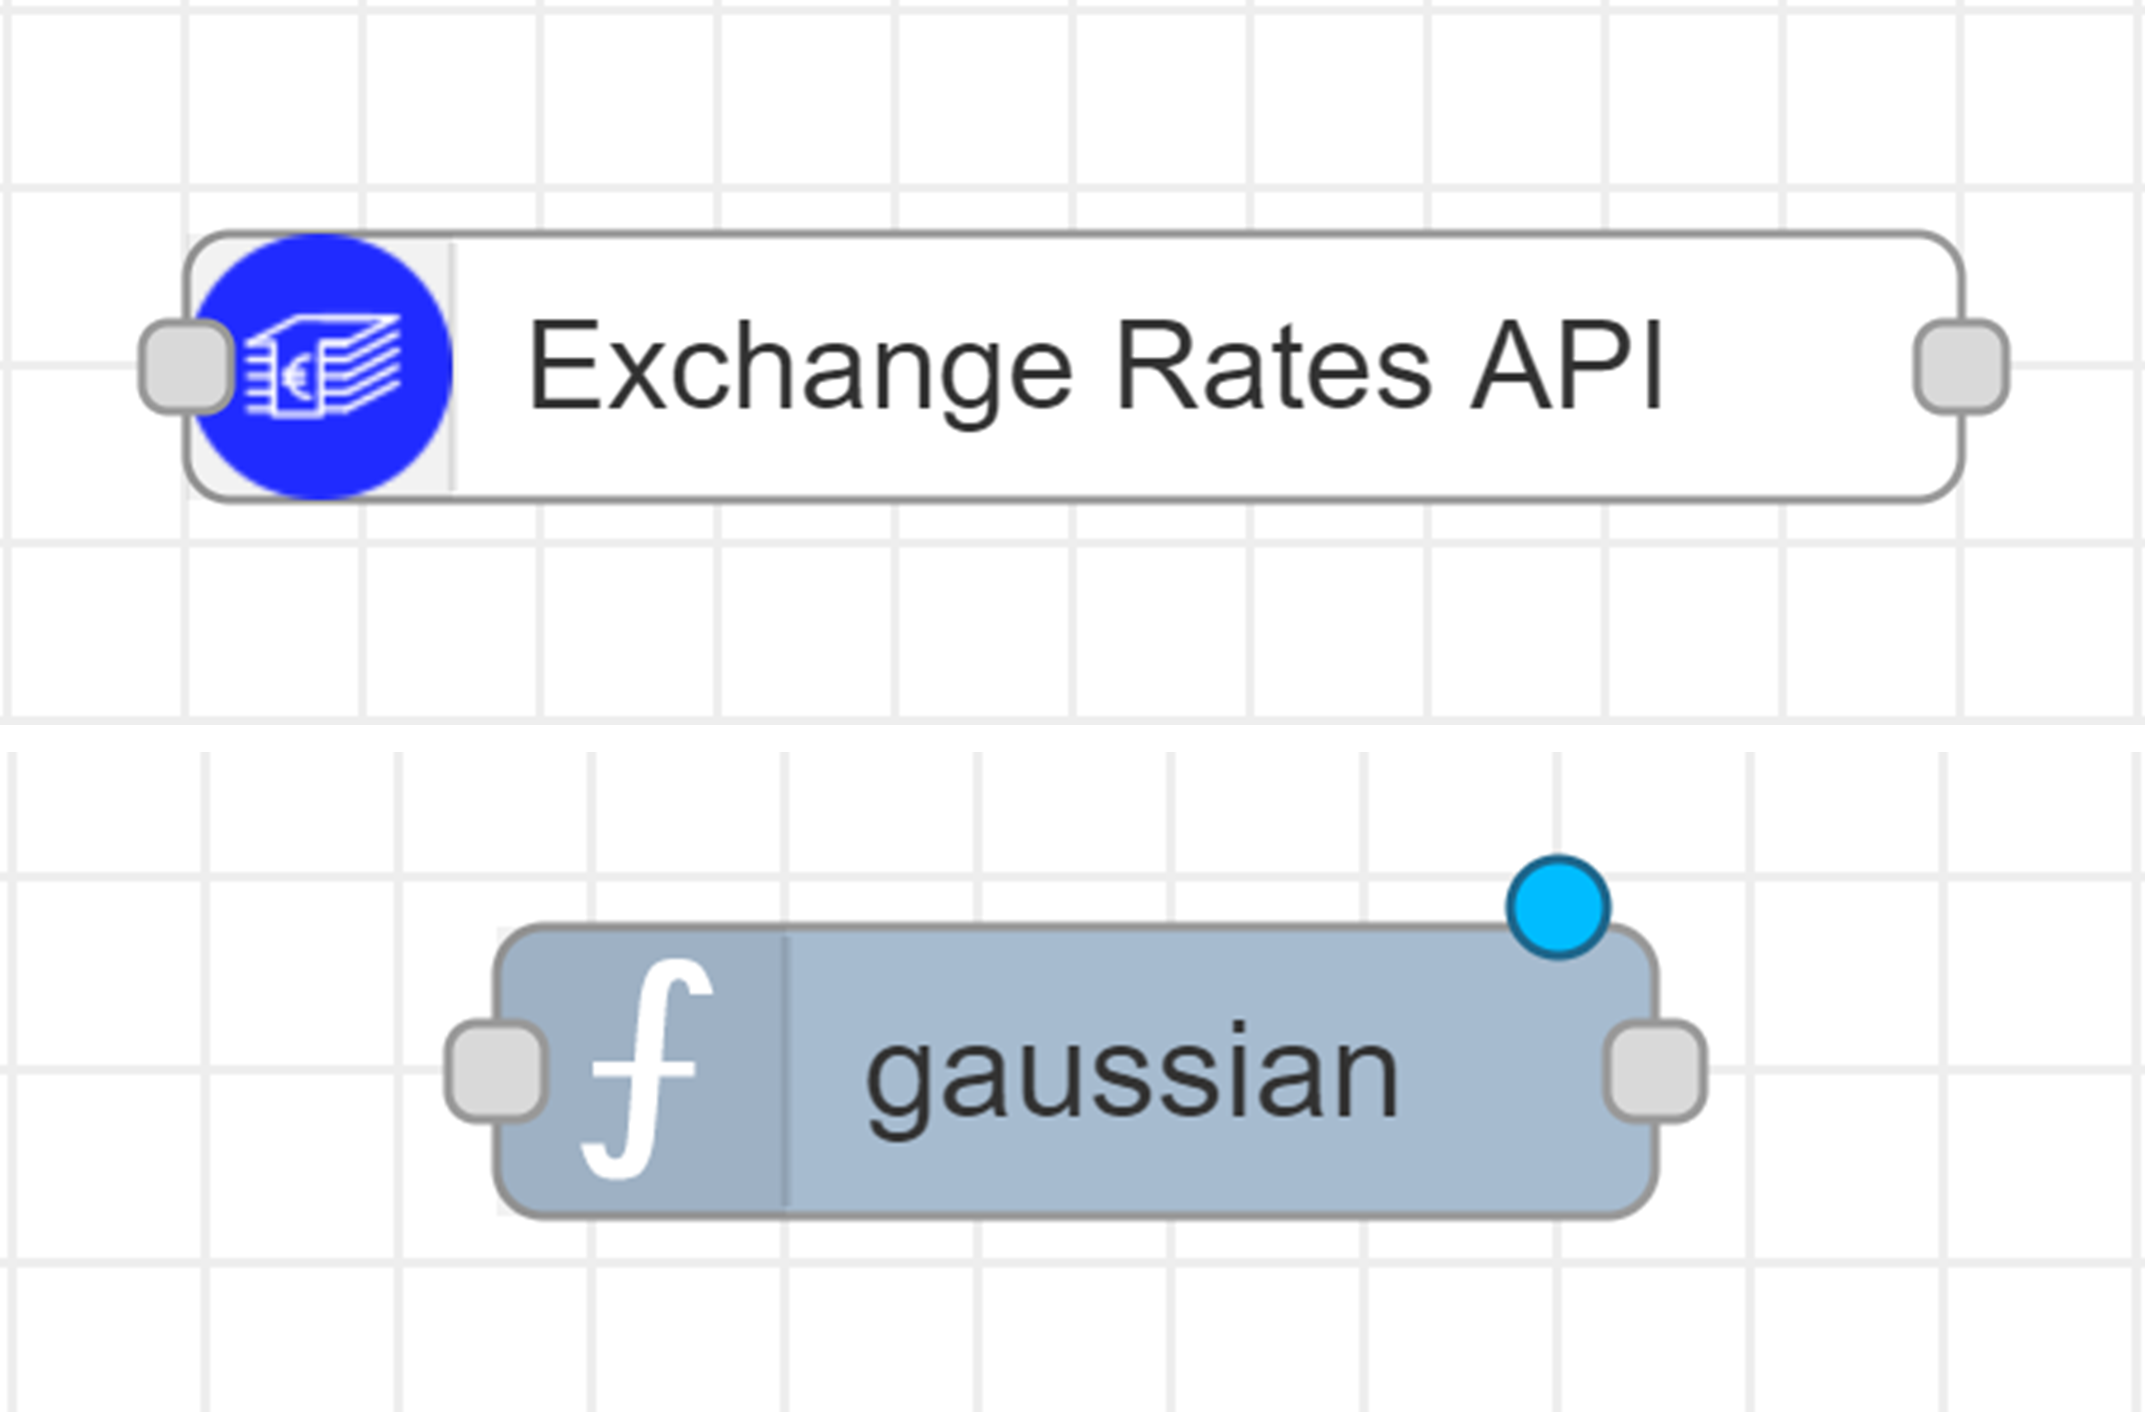
\includegraphics[width=0.3\textwidth]{images/apinodes.png}
    \caption{ Exchange rate API node and Gaussian value generating node}
    \label{fig:apinodes}
\end{figure}

Hence, for the purpose of designing a prototype for this application, we have used the free package which updates the exchange rates hourly. Further, we used a random number generator to vary the hourly rate at 30 second intervals so that only its 5th decimal place varies (which is similar to the real variations of exchange rates every 30 seconds) to simulate the actual variation of exchange rates. These were simulated using Node-RED, and the following packages were used.\\

\textbf{a. node-red-contrib-exchangeratesapi \cite{api}}\\

The base currency and the currency of which the exchange rate is required needs to be specified to this node and it sends an API request to retrieve the required exchange rates. The response from this API containing a large collection of exchange rates is shown in figure \ref{fig:exapi}, from which 6 currency types are selected for our application.\\

A timer was created using the “Inject” node with repeat enabled at hourly intervals to simulate this function.\\

\textbf{b. node-red-contrib-acoustics \cite{acoustics}}\\

The gaussian node from this package (check figure) takes the mean and standard deviation values as inputs and gives a random number as the output. This value was multiplied by the exchange rate in the previous hour and divided by 105to simulate the actual variations of exchange rates every 30 seconds.\\

A timer was created using the “Inject” node with repeat enabled at 30 second intervals to simulate this function.


\subsubsection{Integrating Firebase}

\begin{figure}[H]
    \centering
      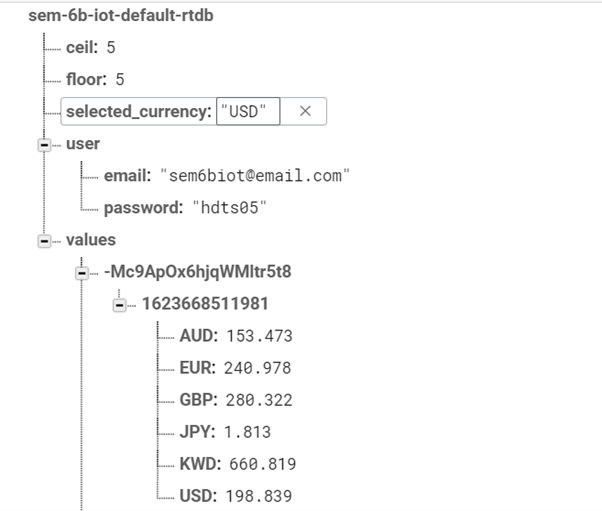
\includegraphics[width=0.5\textwidth]{images/fire.png}
    \caption{Firebase data structure}
    \label{fig:fire}
\end{figure}

The data obtained hourly through API requests, is stored in a Firebase realtime database \cite{firebase} for future use, as there are no free sources of historical exchange rate data for Day Traders. This functionality was implemented via Node-RED as well using the node-red-contrib-firebase \cite{noderedfire} package.\\

Firebase is able to synchronize data to all its connected clients within milliseconds i.e., any change to the database would be reflected in its applications without the need for HTTP requests. Further, the applications hosted using firebase remain interactive, even when the devices are offline, and synchronizes with the database as soon as connectivity is established.\\

The Firebase realtime database is a cloud-hosted database, and one of the many products and services of Google. This is a NoSQL database and hence the data is stored in JSON format. Figure \ref{fig:fire} shows the structure which was used to store the user data, user ceiling / floor values, and the exchange rates in the Firebase realtime database.\\

Three nodes from the node-red-contrib-firebase package have been used to connect the Firebase Realtime database to the Node-RED application, and they are as follows.\\

\textbf{a. firebase.on}\\

This node listens for changes in the database actively and in realtime and takes any changes to the Node-RED application. This was used to synchronize the ceiling and floor values in the database to the Node-RED application in this project.\\

\textbf{b. firebase.once} \\

This node allows us to read data from the database. This was used to extract the exchange rates over 40 hours when plotting the charts of the Node-RED live dashboard.\\

\textbf{c. firebase.modify}\\

This node is used to write or modify the data in the database using the Node-RED application. This was used when storing the authentication data and exchange rate data in the database.\\

\begin{figure}[H]
    \centering
      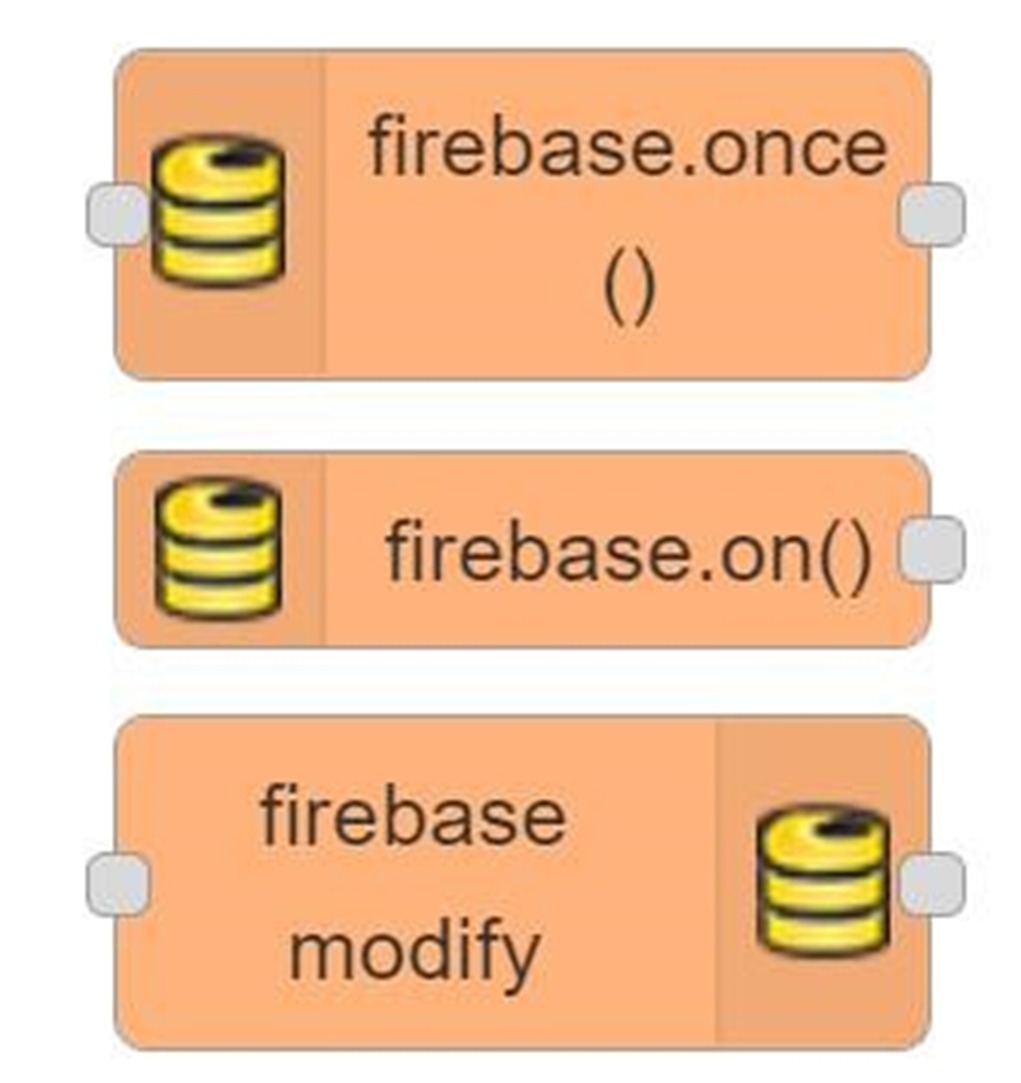
\includegraphics[width=0.7\textwidth]{images/firenodes.png}
    \caption{Firebase nodes used in the project}
    \label{fig:firenodes}
\end{figure}

Following items are saved in Firebase,

\begin{itemize}[itemsep=-1.7mm]
\item User credentials
\item User inputs : selected currency, ceil, floor
\item Fetched hourly foreign exchange rates
\end{itemize}


This is important because the stored data must be available in case of the following situations,

\begin{itemize}[itemsep=-1.7mm]
\item In case the NodeMCU resets
\item In case the Node-RED server restarts
\item To store formatted data into database and fetch later  
\end{itemize}

\subsubsection{Obtaining technical analysis charts from prices}

The hourly price data collected and stored in the real-time database can be sent through popular technical analysis functions to generate useful charts. These charts can be used to make valuable inferences. To process the price data available, an external library named TechnicalIndicators was used. Using the library, following indicators are calculated for hourly historical currency rates. Each currency will have four technical analysis charts.\\


\begin{enumerate}[itemsep=-1.7mm]
\item \textbf{Moving average lines} are frequently used to smooth the fluctuations in a price chart (or a chart of any time series). A moving average is simply the mean of the last n closing prices.

\item \textbf{Rate of Change oscillator} (ROC) or momentum oscillator is calculated as 100 times the difference between the latest closing price and the closing price n periods earlier. Thus, it oscillates around zero.

\item \textbf{Moving average convergence/divergence} (MACD) oscillators are drawn using exponentially smoothed moving averages, which place greater weight on more recent observations. The “MACD line” is the difference between two exponentially smoothed moving averages of the price.

\item \textbf{Relative Strength Index} (RSI) is based on the ratio of total price increases to total price decreases over a selected number of periods. This ratio is then scaled to oscillate between 0 and 100.
\end{enumerate}

\subsubsection{Creating the Node-RED dashboard}

The exchange rate data obtained from the API were analyzed using Node-RED functions to yield the above values of technical indicators over a period of 40 hours and plotted using a Node-RED dashboard as shown in the figure \ref{fig:MACD},\ref{fig:SMA},\ref{fig:ROC} and \ref{fig:RSI}.

\begin{figure}[H]
    \centering
      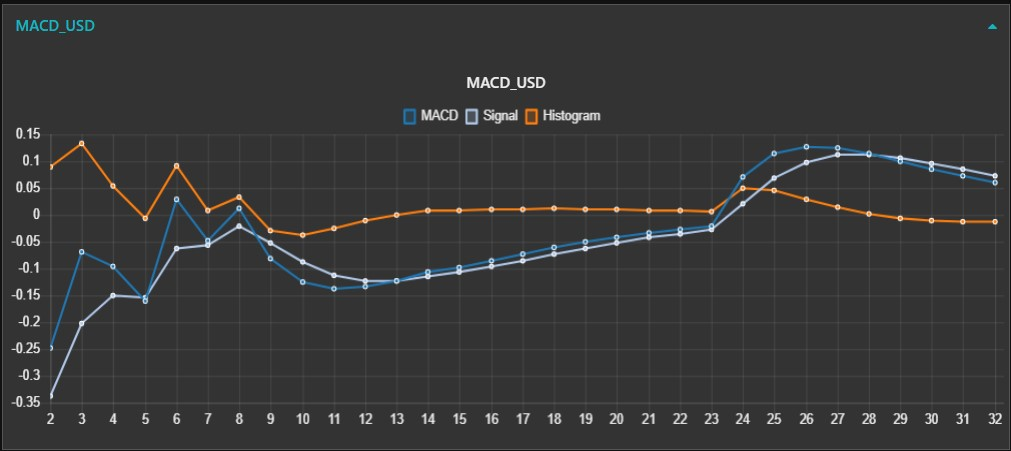
\includegraphics[width=1\textwidth]{images/MACD.jpg}
    \caption{MACD indicator in Node-RED dashboard}
    \label{fig:MACD}
\end{figure}

\begin{figure}[H]
    \centering
      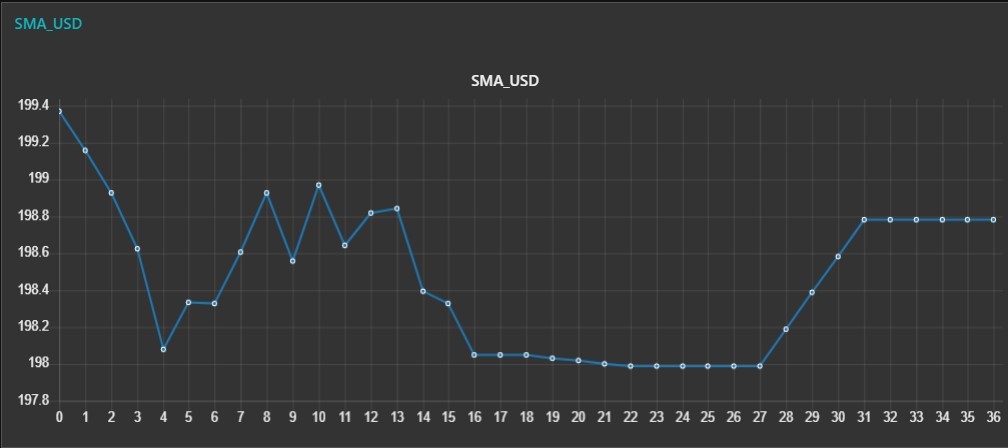
\includegraphics[width=1\textwidth]{images/SMA.jpg}
    \caption{SMA indicator in Node-RED dashboard}
    \label{fig:SMA}
\end{figure}

\begin{figure}[H]
    \centering
      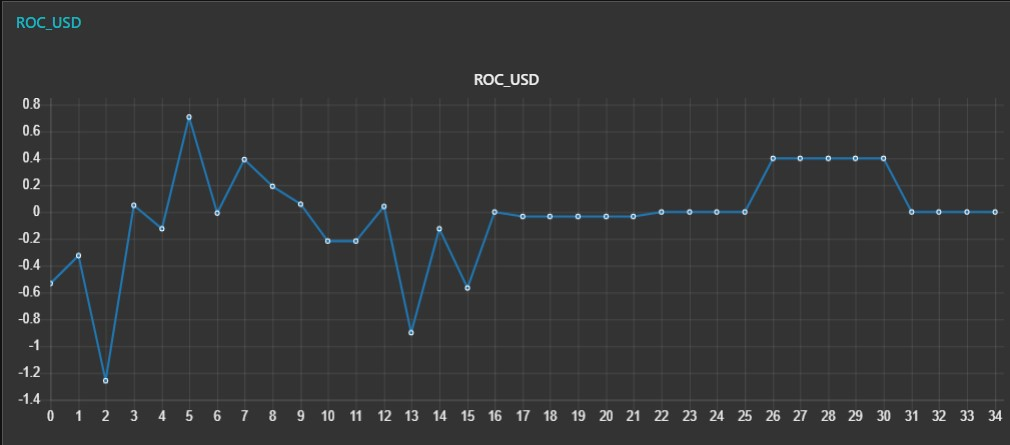
\includegraphics[width=1\textwidth]{images/ROC.jpg}
    \caption{ROC indicator in Node-RED dashboard}
    \label{fig:ROC}
\end{figure}

\begin{figure}[H]
    \centering
      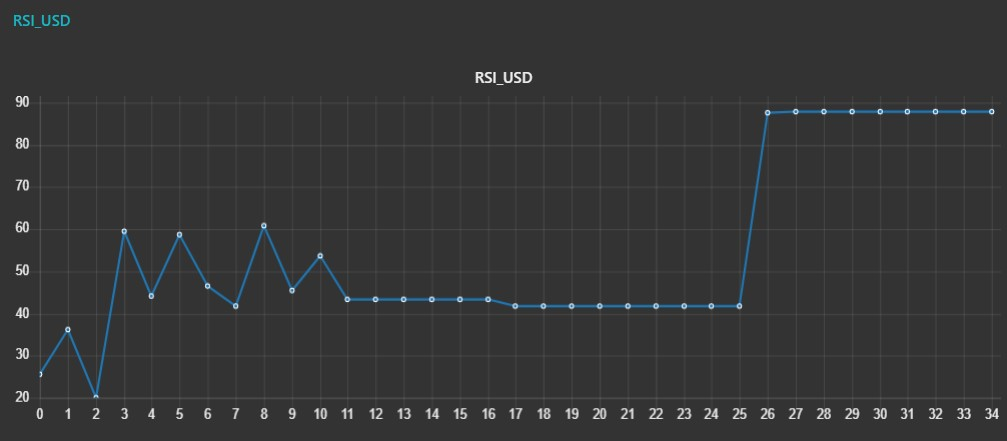
\includegraphics[width=1\textwidth]{images/RSI.jpg}
    \caption{RSI indicator in Node-RED dashboard}
    \label{fig:RSI}
\end{figure}

The dashboard contains 6 Tabs, one for each currency type and 4 groups per tab. Each group contains the plot of  a single technical indicator. The Day Trader can predict the future fluctuations of exchange rates by viewing these charts and making decisions on his future investments. If the exchange rates are going to increase in time to come, he would purchase more currency, and if they are to decrease, he would short sell the currency in his possession.


\section{Results and Discussion}



\section{Conclusion}
%\newpage
\section{Introduction}

\subsection{Overview}

Foreign exchange market is a global market, where people around the world buy and sell different foreign currencies everyday for various purposes. One purpose of the traders in the market is engaging in day-trading activities. Day trading is performed by normal people who intend to obtain profits and earn out of small price mismatches that are available for a short amount of time. Day traders’ activity is influenced by information generated from past foreign currency price information. This information is generated by performing various kinds of mathematical transformations on time series price charts . These people find a lot of value in this information generated and they usually buy required market information from their trusted services.

This project mainly focuses on providing foreign exchange market day-traders, a selected set of useful information. This is achieved by using a currency API that provides live currency prices of various currencies around the world. Usually, hourly past currency price data are not available easily, because past currency data is usually provided on a daily basis. Due to this reason, storing the live currency data in the database is useful for making predictions. Users will also find the notification system that warns when the prices are beginning to exceed their expected boundaries, valuable.

ESP8266 is used for controlling the display as well as connecting to the user’s mobile phone and Node-Red through WiFi technology. Node-Red to Node-MCU communication happens through the MQTT communication protocol. Node-MCU’s ability to enter into sleep mode is also utilized. Node-MCU acts as both Wifi access point and http server. The user may sign-in using a username and a password, when the Node-MCU is functioning as a server. The access point mode is required when it is fetching and submitting data.


\subsection{Objectives}

\begin{itemize}[itemsep=-1.7mm]

\item To provide several technical analysis charts such as Simple Moving Average \item to the day-trader so that they can make useful predictions
\item To provide the useful information in a user friendly manner through the Node-Red dashboard as well as mobile interface.
\item To notify and alarm the day-trader clients when their set upper and lower boundaries are exceeded so that they can take quick actions.
\item To provide the user flexibility to choose the interested currencies for observation


\end{itemize}


\subsection{Scope}

The scope of the project is to build an innovative IOT application using IOT concepts, tools and standards available. The basic architecture should include a realtime database, an open-source API, Node-Red, Node-MCU and a client mobile phone. Use of a communication protocol such as CoAP or MQTT is also encouraged.


\subsection{Architecture}

\begin{figure}[h]
    \centering
      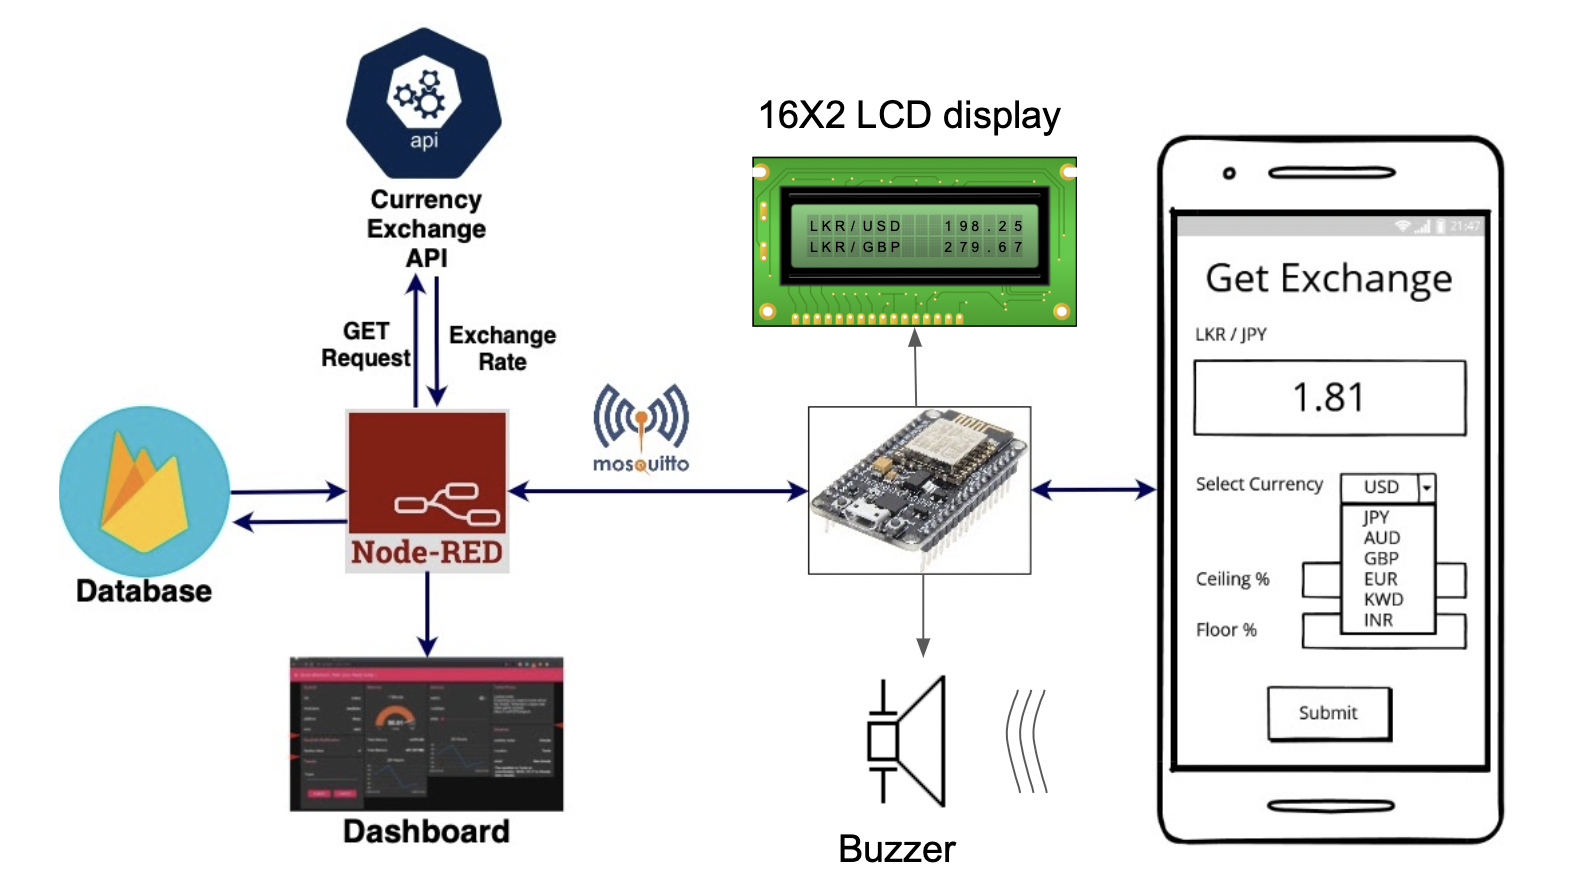
\includegraphics[width=1\textwidth]{images/arch.png}
    \caption{Architecture of Currency Converter Service}
    \label{fig:orgchart}
\end{figure}

\newpage
\bibliographystyle{IEEEbib}
\bibliography{references}


\newpage
\section{Annexes}

\subsection{ESP8266 code}
                
\begin{lstlisting}[language=C++]
{
#if defined(ESP8266)
#include <ESP8266WiFi.h>          
#else
#include <WiFi.h>          
#endif

#if defined(ESP8266)
#include <ESP8266WebServer.h>
#else
#include <WebServer.h>
#endif

#include <WiFiManager.h> 
#include <DNSServer.h>
#include <PubSubClient.h>

#include <WiFiUdp.h>
#include <NTPClient.h>               
#include <TimeLib.h>                 
#include <LiquidCrystal.h>  
LiquidCrystal lcd(D6, D5, D1, D2, D3, D4); 

ESP8266WebServer server(80);

WiFiClient wifiClient;
PubSubClient client(wifiClient); 
const char* mqttServer = "test.mosquitto.org";

// Setup NTP for time and date
WiFiUDP ntpUDP;
NTPClient timeClient(ntpUDP, "asia.pool.ntp.org", 19800, 60000);
char Time[ ] = "TIME:00:00:00";
char Date[ ] = "DATE:00/00/2000";
byte last_second, second_, minute_, hour_, day_, month_;
int year_;
int counter = 0;
unsigned long unix_epoch;
char ascii;

// Node MCU expects from Node-red per 15 seconds
//1) All six currencies values and up/down status ( in the order USD, KWD, AUD, EUR, JPY, GBP)
//2) Selected currency of the user
//3) floor or ceiling exceeded (true/false)


// Node Red expects from Node MCU
//1) Clients selected Currency type
//2) Ceil and Floor of the currency type as percentages (eg-:5,4)
String payloadstr;
unsigned long timestamp;

float USD = 198.25; // up - true, down - false
float GBP = 198.25; // up - true, down - false
float JPY = 198.25; // up - true, down - false
float AUD = 198.25; // up - true, down - false
float KWD = 198.25; // up - true, down - false
float EUR = 198.25; // up - true, down - false

bool usd_up = false;
bool gbp_up = false;
bool jpy_up = false;
bool aud_up = false;
bool kwd_up = false;
bool eur_up = false;
char * binary;

String current_user;
String current_currency;
bool ceil_crossed = false;
bool floor_crossed = false;

//Variables required for buzzer sound
int speakerPin = 13;
int len = 15; // the number of notes
char notes[] = " C C C C C C C C C ";// a space represents a rest
int beats[] = { 1,1, 1, 1, 1, 1, 1, 1, 1, 1, 1, 1, 1, 1, 1, 1, 1, 1, 1 };
int tempo = 300;


void setup_wifi() {
  // Connecting to a WiFi network
  delay(5000);
  WiFiManager wifiManager; 
  wifiManager.autoConnect("IoT6B_G05","12345678");
}

void setupMQTT() {
  client.setServer(mqttServer,1883);
  client.setCallback(callback);
  }

void reconnect() {
  // Loop until we're reconnected
  while (!client.connected()) {
    Serial.print("Attempting MQTT connection...");
    // Create a random client ID
    String clientId = "ESP32Client-";
    clientId += String(random(0xffff), HEX);
    // Attempt to connect
    if (client.connect(clientId.c_str())) {
      Serial.println("connected");
      // Once connected, publish an announcement...
      client.publish("IOT_6B/G05/start", "Hello World");
      // ... and resubscribe
      client.subscribe("IOT_6B/G05/BuzzerNotification");
      client.subscribe("IOT_6B/G05/CommonData");
    } else {
      Serial.print("failed, rc=");
      Serial.print(client.state());
      Serial.println(" try again in 500 milli seconds");
      // Wait 5 seconds before retrying
      delay(500);
    }
  }
}

void setup() {
  // put your setup code here, to run once:
  
  lcd.begin(16, 2);                 // Initialize 16x2 LCD Display
  lcd.clear();
  lcd.setCursor(0, 0);
  lcd.print(Time);
  lcd.setCursor(0, 1);
  lcd.print(Date);
  timeClient.begin();

  pinMode(speakerPin, OUTPUT);  // Output pin for buzzer
  
  pinMode(BUILTIN_LED, OUTPUT);     // Initialize the BUILTIN_LED pin as an output
  WiFi.mode(WIFI_AP_STA);
  Serial.begin(115200);
  setup_wifi();
  setupMQTT();

  //client.subscribe("IOT_6B/G05/Response");
  //client.subscribe("IOT_6B/G05/ceil");
  
  server.on("/",handlerequest);
  server.onNotFound(handle_NotFound);

  server.begin();
  Serial.println("HTTP server started");

}

void loop() {
  server.handleClient();
  if (!client.connected()) {
    reconnect();
  }
  client.loop();

    timeClient.update();
  unix_epoch = timeClient.getEpochTime();    // Get Unix epoch time from the NTP server
  //Serial.println(unix_epoch);
  second_ = second(unix_epoch);
  if (last_second != second_) {
 

    minute_ = minute(unix_epoch);
    hour_   = hour(unix_epoch);
    day_    = day(unix_epoch);
    month_  = month(unix_epoch);
    year_   = year(unix_epoch);

    Time[12] = second_ % 10 + 48;
    Time[11] = second_ / 10 + 48;
    Time[9]  = minute_ % 10 + 48;
    Time[8]  = minute_ / 10 + 48;
    Time[6]  = hour_   % 10 + 48;
    Time[5]  = hour_   / 10 + 48;

    Date[5]  = day_   / 10 + 48;
    Date[6]  = day_   % 10 + 48;
    Date[8]  = month_  / 10 + 48;
    Date[9]  = month_  % 10 + 48;
    Date[13] = (year_   / 10) % 10 + 48;
    Date[14] = year_   % 10 % 10 + 48;

    //Serial.println(Time);
    //Serial.println(Date);

    lcd.setCursor(0, 0);
    lcd.print(Time);
    lcd.setCursor(0, 1);
    lcd.print(Date);
    last_second = second_;

  }
  delay(500);

  if (counter == 8){
    counter = 0;
    lcd.setCursor(0, 0);
    lcd.print("LKR/USD "+ String(USD));
    lcd.setCursor(0, 1);
    lcd.print("LKR/GBP "+ String(GBP));

    if (usd_up){
      ascii = 0x5e;
      lcd.setCursor(15 , 0);
      lcd.print(ascii);
    } else {
      ascii = 0x76;
      lcd.setCursor(15 , 0);
      lcd.print(ascii);
    }

    if (gbp_up){
      ascii = 0x5e;
      lcd.setCursor(15 , 1);
      lcd.print(ascii);
    } else {
      ascii = 0x76;
      lcd.setCursor(15 , 1);
      lcd.print(ascii);
    }
    delay(2000);

    server.handleClient();
    client.loop();

    
    lcd.clear();
    lcd.setCursor(0, 0);
    lcd.print("LKR/JPY   "+ String(JPY));
    lcd.setCursor(0, 1);
    lcd.print("LKR/AUD "+ String(AUD));

    if (jpy_up){
      ascii = 0x5e;
      lcd.setCursor(15 , 0);
      lcd.print(ascii);
    } else {
      ascii = 0x76;
      lcd.setCursor(15 , 0);
      lcd.print(ascii);
    }

    if (aud_up){
      ascii = 0x5e;
      lcd.setCursor(15 , 1);
      lcd.print(ascii);
    } else {
      ascii = 0x76;
      lcd.setCursor(15 , 1);
      lcd.print(ascii);
    }
    delay(2000);

    server.handleClient();
    client.loop();
    lcd.clear();
    lcd.setCursor(0, 0);
    lcd.print("LKR/KWD "+ String(KWD));
    lcd.setCursor(0, 1);
    lcd.print("LKR/EUR "+ String(EUR));

    if (kwd_up){
      ascii = 0x5e;
      lcd.setCursor(15 , 0);
      lcd.print(ascii);
    } else {
      ascii = 0x76;
      lcd.setCursor(15 , 0);
      lcd.print(ascii);
    }

    if (eur_up){
      ascii = 0x5e;
      lcd.setCursor(15 , 1);
      lcd.print(ascii);
    } else {
      ascii = 0x76;
      lcd.setCursor(15 , 1);
      lcd.print(ascii);
    }

    delay(2000);
    server.handleClient();
    client.loop();
    lcd.clear();
  } else {
    counter += 1;
  }

}

void handlerequest(){
//  if (server.hasArg("plain")== false){ //Check if body received
//      server.send(200, "text/plain", "Body not received");
//      return;
//      }
      String UserNeeds;
      current_currency = server.arg("currency");
      String Ceil = server.arg("ceil");
      String Floor = server.arg("floor");
      unsigned long timenow = unix_epoch - 19800;

      UserNeeds  = timenow + "$" + current_currency +"$"+ Ceil +"$"+ Floor;



      int currency_len = current_currency.length() ;
      int ceil_len = Ceil.length();
      int floor_len = Floor.length(); 
      
      int UserNeeds_len = currency_len + ceil_len + floor_len +3;

      char UserNeeds_array[UserNeeds_len];
      UserNeeds.toCharArray(UserNeeds_array, UserNeeds_len);
      client.publish("IOT_6B/G05/UserNeeds", UserNeeds_array );


      server.send(200, "text/html", SendHTML(current_currency));
}

void handle_NotFound(){
  server.send(404, "text/plain", "Not found");
}

String SendHTML(String Currency){
  String ptr = "<!DOCTYPE html> <html lang=\"en\">\n";
  ptr+= "<head>\n";
  ptr+= "<link rel=\"stylesheet\" href=\"https://cdnjs.cloudflare.com/ajax/libs/font-awesome/4.7.0/css/font-awesome.min.css\">\n";   
  ptr+= "<meta charset=\"UTF-8\">\n";
  ptr+= "<meta http-equiv=\"X-UA-Compatible\" content=\"IE=edge\">\n";
  ptr+= "<meta name=\"viewport\" content=\"width=device-width, initial-scale=1.0\">\n";
  ptr+= "<title>GROUP 5</title>\n";
  ptr+= "</head>\n";
  ptr+= "<body style=\"text-align:center;display:grid;place-content: center;background-color: rgb(23, 196, 196);\"\n";
  ptr+= "<h1 style=\"font-size: 200px;\" >Get Exchange</h1>\n";
  
  if (Currency == "USD"){
    ptr+="<h2>LKR/USD</h2>\n";
  }
  else if (Currency == "JPY"){
    ptr+="<h2>LKR/JPY</h2>\n";
  }
  else if (Currency == "GBP"){
    ptr+="<h2>LKR/GBP</h2>\n";
  }
  else if (Currency == "EUR"){
    ptr+="<h2>LKR/EUR</h2>\n";
  }
  else if (Currency == "KWD"){
    ptr+="<h2>LKR/KWD</h2>\n";
  }
  else if (Currency == "INR"){
    ptr+="<h2>LKR/INR</h2>\n";
  }
  else{
    ptr+="<h2>LKR/NON</h2>\n";
  }
  
  ptr+= "<h1 style=\" color :rgb(62, 128, 0)\">1.81 <i class=\"fa fa-arrow-up\"></i></h1>\n";
  ptr+= "<h1 style=\" color :red\">1.81 <i class=\"fa fa-arrow-down\"></i></h1>\n";
  ptr+= "<form name=\"dropdown\" method=\"get\" style=\" font-size: xx-large;\" >\n";
  ptr+= "<label for=\"currency_label\">Select Currency :</label><br>\n";
  ptr+= "<select name=\"currency\" id=\"currency\">\n";
  ptr+= "<option value=\"USD\">USD</option>\n";
  ptr+= "<option value=\"JPY\">JPY</option>\n";
  ptr+= "<option value=\"GBP\">GBP</option>\n";
  ptr+= "<option value=\"EUR\">EUR</option>\n";
  ptr+= "<option value=\"KWD\">KWD</option>\n";
  ptr+= "<option value=\"INR\">INR</option>\n";
  ptr+= "</select>\n";
  ptr+= "<br><br>\n";
  ptr+= "<label for=\"ceil\">Ceil% :</label><br>\n";
  ptr+= "<input type=\"number\" id=\"ceil\" name=\"ceil\" value=5><br><br>\n";
  ptr+= "<label for=\"floor\">Floor% :</label><br>\n";
  ptr+= "<input type=\"number\" id=\"floor\" name=\"floor\" value=5><br><br>\n";
  ptr+= "<input type=\"submit\" value=\"Submit\">\n";
  ptr+= "</form>\n";
  ptr+= "</body>\n";
  ptr+= "</html>\n";
  return ptr;
}

void callback(char* topic, byte* payload, unsigned int length) {

  if (String(topic) == "IOT_6B/G05/BuzzerNotification") {
   process_notification(payload, length, 50, 5);
  }
  
  if (String(topic) == "IOT_6B/G05/CommonData") {
   process_data(payload, length, 70, 8);
  }

  if (ceil_crossed  || floor_crossed) {
    buzzerinit();  
    ceil_crossed = false;
    floor_crossed = false;
  }
}

void process_notification(byte* payload, unsigned int length, int charlen, int numitem) {

    int digit;
    payloadstr = "";
    Serial.println();
    for (int i = 0; i < length; i++) {
      payloadstr += (char)payload[i];
    }

     char payloadstr_array[charlen];
     payloadstr.toCharArray(payloadstr_array, charlen);

   char * token = strtok(payloadstr_array, "$");
   
   for (int i = 1; i < numitem+1; i++) {
      switch (i) {
       case 1:
          timestamp = atol(token);
          Serial.print(timestamp);
          Serial.println();
          break;
       case 2:
          if (timestamp > unix_epoch - 19820) {
           current_user = String(token);
           Serial.print(current_user);
           Serial.println();
          }
           break;
       case 3:
          if (timestamp > unix_epoch - 19820) {
           current_currency = String(token);
           Serial.print(current_currency);
           Serial.println();
          }
           break;
       case 4:
          if (timestamp > unix_epoch - 19820) {
           digit = String(token).toInt();
           if (digit == 1) {
           ceil_crossed = true;
            } else {
            ceil_crossed  = false;
            }
           Serial.print(ceil_crossed);
           Serial.println();
          }
          break;
       case 5:
          if (timestamp > unix_epoch - 19820) {
           digit = String(token).toInt();
           if (digit == 1) {
           floor_crossed = true;
            } else {
           floor_crossed  = false;
            }
           Serial.print(ceil_crossed);
           Serial.println();
          }
          break;    
       }
       token = strtok(NULL, "$");
   }
}

void process_data(byte* payload, unsigned int length, int charlen, int numitem) {

    payloadstr = "";
    Serial.println();
    for (int i = 0; i < length; i++) {
      payloadstr += (char)payload[i];
    }

     char payloadstr_array[charlen];
     payloadstr.toCharArray(payloadstr_array, charlen);

   char * token = strtok(payloadstr_array, "$");

   for (int i = 1; i < numitem+1; i++) {
      switch (i) {
       case 1:
          timestamp = atol(token);
          Serial.print(timestamp);
          Serial.println();
          break;
       case 2:

           USD = String(token).toFloat();
           Serial.print(USD);
           Serial.println();
           break;
       case 3:

           GBP = String(token).toFloat();
           Serial.print(GBP);
           Serial.println();
           break;
       case 4:

           JPY = String(token).toFloat();
           Serial.print(JPY);
           Serial.println();
          break;
       case 5:

           AUD = String(token).toFloat();
           Serial.print(AUD);
           Serial.println();
          break;
       case 6:
          //do something when var equals 1
           KWD = String(token).toFloat();
           Serial.print(KWD);
           Serial.println();
          break;
       case 7:

           EUR = String(token).toFloat();
           Serial.print(EUR);
           Serial.println();
          break;
       case 8:
           set_updown(token);
           break;        
       }
       token = strtok(NULL, "$");
   }

}

void set_updown(char * binary) {
  int digit;
  for (int i = 1; i < 7; i++) {
    switch (i) {
       case 1:
       digit = String((char)binary[i-1]).toInt();
       if (digit == 1) {
        usd_up = true;
       } else {
        usd_up = false;
       }
       Serial.print(usd_up);
       Serial.println();
       break;

       case 2:
       digit = String((char)binary[i-1]).toInt();
       if (digit == 1) {
        gbp_up = true;
       } else {
        gbp_up = false;
       }
       Serial.print(gbp_up);
       Serial.println();
       break;

       case 3:
       digit = String((char)binary[i-1]).toInt();
       if (digit == 1) {
        jpy_up = true;
       } else {
        jpy_up = false;
       }
       Serial.print(jpy_up);
       Serial.println();
       break;

       case 4:
       digit = String((char)binary[i-1]).toInt();
       if (digit == 1) {
        aud_up = true;
       } else {
        aud_up = false;
       }
       Serial.print(aud_up);
       Serial.println();
       break;

       case 5:
       digit = String((char)binary[i-1]).toInt();
       if (digit == 1) {
        kwd_up = true;
       } else {
        kwd_up = false;
       }
       Serial.print(kwd_up);
       Serial.println();
       break;

       case 6:
       digit = String((char)binary[i-1]).toInt();
       if (digit == 1) {
        eur_up = true;
       } else {
        eur_up = false;
       }
       Serial.print(eur_up);
       Serial.println();
       break;
    }
  }
}

void playTone(int tone, int duration) {
  for (long i = 0; i < duration * 1000L; i += tone * 2) {
    digitalWrite(speakerPin, HIGH);
    delayMicroseconds(tone);
    digitalWrite(speakerPin, LOW);
    delayMicroseconds(tone);
  }
}

void playNote(char note, int duration) {
  char names[] = { 'c', 'd', 'e', 'f', 'g', 'a', 'b', 'C' };
  int tones[] = { 1915, 1700, 1519, 1432, 1275, 1136, 1014, 956 };

  // play the tone corresponding to the note name
  for (int i = 0; i < 8; i++) {
    if (names[i] == note) {
      playTone(tones[i], duration);
    }
  }
}

void buzzerinit() {
  for (int i = 0; i < len; i++) {
    if (notes[i] == ' ') {
      delay(beats[i] * tempo); // rest
    } else {
      playNote(notes[i], beats[i] * tempo);
    }

    // pause between notes
    delay(tempo / 2); 
  }
}
}
\end{lstlisting}

\subsection{JavaScript codes used in Node-Red}




\end{document}
